\chapter{State of the Art} \label{chap:State of the Art}
% introduction

\section{Implementation of Reactive Systems}
	\subsection{Reactive Programming}
	% eventStreams
	% observables, difference to Observer design pattern.
	
	\subsection{RxJs and BaconJs}
	% Though there are other Javascript implementations of the reactive design pattern like https://github.com/stoeffel/awesome-frp-js,
	% kefir, cyclejs
	% this thesis focuses on RxJs and BaconJs, because these are the one the extension currently supports.
	
	%RXjs
	%var button = document.querySelector('button');
	%Rx.Observable.fromEvent(button, 'click')
	%.throttleTime(1000)
	%.scan(count => count + 1, 0)
	%.subscribe(count => console.log(`Clicked ${count} times`));
	% The essential concepts in RxJS which solve async event management are:
	%Observable: represents the idea of an invokable collection of future values or events.
	%Observer: is a collection of callbacks that knows how to listen to values delivered by the Observable.
	%Subscription: represents the execution of an Observable, is primarily useful for cancelling the execution.
	%Operators: are pure functions that enable a functional programming style of dealing with collections with operations like map, filter, concat, flatMap, etc.
	%Subject: is the equivalent to an EventEmitter, and the only way of multicasting a value or event to multiple Observers.
	%Schedulers: are centralized dispatchers to control concurrency, allowing us to coordinate when computation happens on e.g. setTimeout or requestAnimationFrame or others.
	
	
	%Baconjs: 
	%Generally, this is how you implement an app with Bacon.js. Capture input into EventStreams and Properties - Transform and compose signals into ones that describe your domain. - Assign side-effects to signals.
	%EventStreams (distinct events) and Properties (values that change over time). 
	%$("#username input").asEventStream("keyup").map(function(event) { return $(event.target).val() }).toProperty("")

	\subsection{Debugging Reactive Code}
	% other systems that do
	% - Reactive Inspector for scala https://guidosalva.github.io/reactive-inspector/ 
	% - reference to rxfiddle
	% - unit tests and do-debugging for Rx: https://msdn.microsoft.com/en-us/library/hh242967(v=vs.103).aspx to reduce the effort of adding do-statements each time a bug is tracked down, the developer can add logging functionality and use that in the do statement. https://shiny.rstudio.com/articles/debugging.html #"The Reactive log" where a visualization is later used on the log to create a simple dependency graph containing code pieces as nodes.
	


\section{Previous and Related Work}
	\subsection{The Chrome Reactive Inspector}		
		\subsubsection{Master Thesis by Waqas Abbas}
		% main focus of the thesis
		% implemented result of the thesis in short
		
		\subsubsection{Master Thesis by Pradeep Baradur}
		% main focus of the thesis
		% new features introduced
		
		\subsubsection{Merging previous efforts}
		%- took chrome-reactive-inspector 2 as base and merge all later developed features into it, piece by piece.
		% - uncompatible git histories - solvable but not much use since the files had separated so much in text character changes, though not so much in logic -> renames and splitting of files
		% - manually copied changes by Pradeep from Waqas's repository. Hard to detect, changed to match other variable names before committing.
		% - access to many global variables made tracking down dependencies of components hard with mixed contexts - some files with the window object corresponding to contentscripts in the same directory as files with a window object corresponding to the extensions window.
		%TODO: change tone to always present problems as general difficulties instead of shortcomings
		
		\subsubsection{"Special Curicumstances"}
		% demo version of jalangi
		% instrumenting files via scanning the html for script tags
		% -> will not work for module loaders like require.js or ecma6
		% -> will not work with bundled javascript code - but since in development there should be a non bundled version available not 
		% a big problem in javascript. But for Typescript since the extension does not support it and when compiling there may already be bundling in place. (#add some text from future here#)
		
		% Shared context through "new Function" that breaks the separation enforced by chrome. To increase consistency and prevent different execution contexts the previous eval was replaced with "new Function" but this does not reduce the security risk.There are other options to execute scripts from a chrome extension but since some of the extension scripts need to share the Rx or Bacon object with the inspected pages javascript files there is no other way. ofcorse that breaks the normal isloated world and intodruces a new set of problems like conflicting names. The security risk involved in executing a foreign script in a "trusted" extension context could be reduced if a sandbox was used as described in https://developer.chrome.com/extensions/sandboxingEval. Then all the inspected pages content scripts and some special recording scripts could be executed in that sandbox and transmitt the recorded nodes back via message passing.
		% - Dangers of using eval -> execution in current context. if called from other function, "this" might change. Function() for global with window passed to execute in original context.
		%- Note that  files that are not selected for instrumentation will still generate nodes in the graph, because the Rx and Bacon frameworks will still record interactions.
		%- The Bacon and Rx scripts are prevented from loading so the extensions own files can be used. This is accomplished by filtering all referenced js files in the inspected page for any Bacon or Rx library files and excluding them from the loading process. They need to match version exactly though. 
	

	\subsection{RxFiddle}
	% features of RxFiddle
	% limitations: 'one of the limitations of RxFiddle is ... which we tackeld in this work.
	% test rxFiddle with one example that generates thousands of steps


% end of state of the art chapter
%----------------------------------------------------------------------------
%latex sample code:



\begin{figure}[!h]
	\centering
	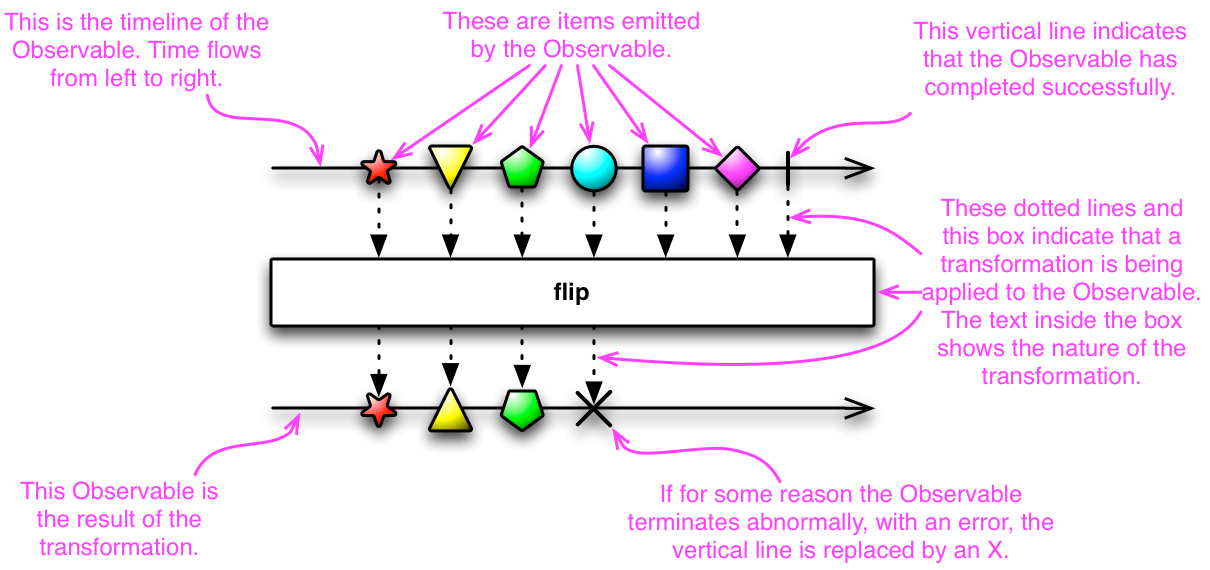
\includegraphics[scale=0.5,trim=0 0 0 0]{gfx/rxjs-reactive-pattern2.png}
	\caption{Reactive pattern \protect\cite{ReactiveXobservable}}
	\label{fig:rxjs-reactive-pattern}
\end{figure}

\textbf{Observable and Observer}\\
Placeholder

\textbf{Operators}
\label{subsec:Operators}\\

\textbf{RxJS Code Structure}\\
Placeholder
\begin{lstlisting}[language=JavaScript, caption=RxJS Simple Example, label={lst:RxJS_Simple_Example}]
// 1. Srouce Observable Creation
var sourceObservable = Rx.Observable.interval(1000);
// 2. Transformation by applying different operators
var transformedObservable = sourceObservable.map(function(x) {
		return x * 10;
	})
	.filter(function(x) {
		return x !== 20
	})
// OUTPUT
Next: 0
Next: 10
Next: 30
Next: 40
Next: 50
Completed
\end{lstlisting}

\subsection{Bacon.js}

\textbf{EventStream and Property}\\
Placeholder

